\documentclass[%
 reprint,
 amsmath,
 amssymb,
 aps,
]{revtex4-2}

\usepackage{graphicx}% Include figure files
\usepackage{dcolumn}% Align table columns on decimal point
\usepackage{bm}% bold math
\usepackage{lipsum}
\usepackage{physics}



\bibliographystyle{apsrev4-2}


\begin{document}

%\preprint{APS/123-QED}
\title{Manuscript Title:\\Sub-Title of manuscript }% Force line breaks with \\

\author{author1}%
 \affiliation{Authors' institution and/or address}%
 \email{email@address.tbd}
\author{author1}%
\affiliation{%
Authors' institution and/or address}%


\date{\today}

\begin{abstract}
\lipsum[1]
\end{abstract}

\maketitle


\section{Section 1}

\lipsum[1-2] Fake citation. Results can be seen in Figs. \ref{fig:image-1}.

\lipsum[1] Fake citation. \cite{chakraborty2020multiphonon}.

\begin{figure}
    \centering
    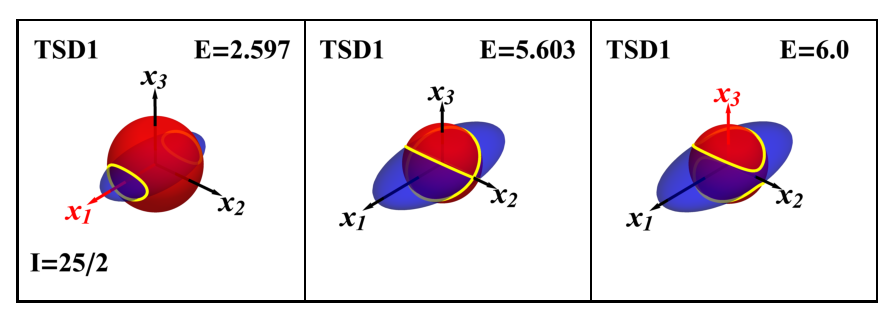
\includegraphics[width=0.45\textwidth]{images/energy_ellipsoids/tsd1_spin1.eps}
    \caption{Image 1}
    \label{fig:image-1}
\end{figure}


\begin{figure}
    \centering
    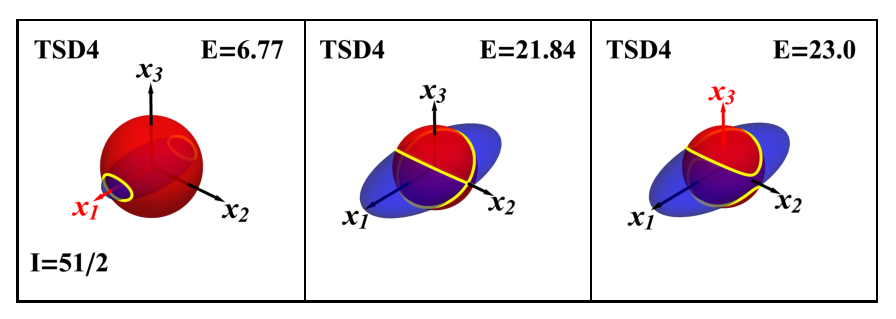
\includegraphics[width=0.45\textwidth]{images/energy_ellipsoids/tsd4_spin2.eps}
    \caption{Image 2}
    \label{fig:image-2}
\end{figure}


\bibliography{biblio}% Produces the bibliography via BibTeX.

\end{document}